\section{更新方法(初次阅读使用可跳过)}

% \subsection{开始之前}

% 若您想要更新到 v1.3.15 及以下版本(不推荐),请阅读本章第 2 小节。
% 若您想要更新到 v1.3.16 及以上版本,请阅读本章第 3 小节。
% v1.3.16 版本自定义功能得到了非常大的提升,更新到 v1.3.16 及以上版本的方法相比于更新到 v1.3.15 之前的版本要简化不少。

% \textbf{\color{red}\lstinline{lua} 目录下的 \lstinline{Setting.lua} 及 \lstinline{WeaponList.lua} 是根据用户自身情况自行定义的配置文件(配置文件一共就这两个)。
% 按照本文档介绍的方式配置完毕能够正常使用后,您应当妥善保管,如若丢失则需要重新配置。}

% \textbf{\color{red}在更新开始前,请先关闭旧版本控制器和 GamingTool。}

% \begin{figure}[H]
%     \Centering
%     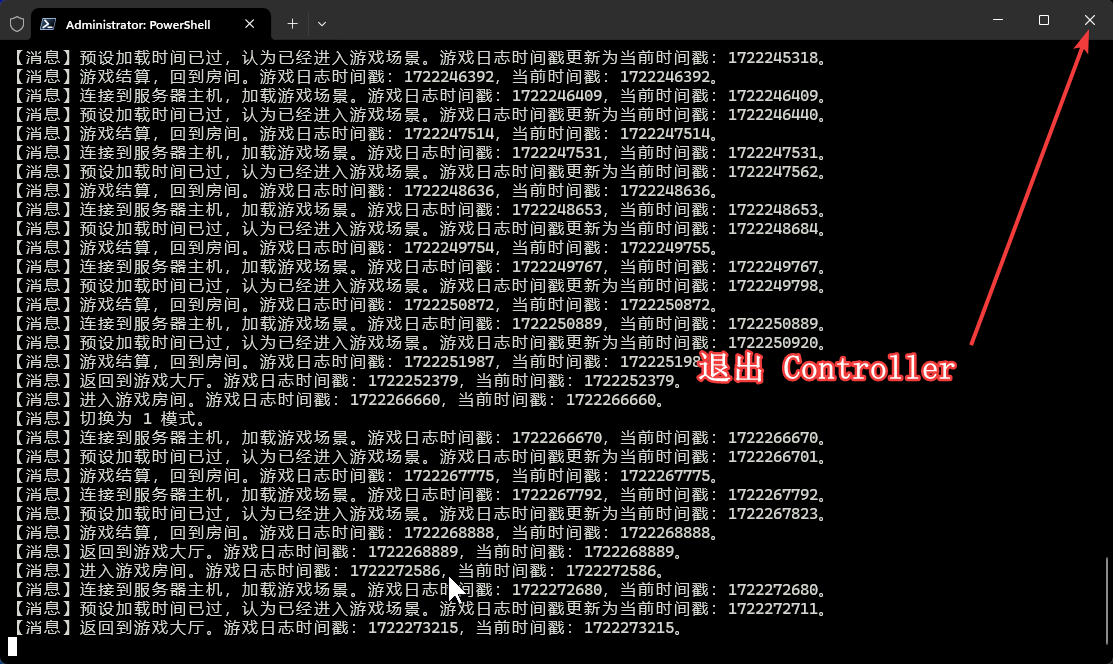
\includegraphics[width=\textwidth]{docs/assets/update/close_controller.png}
%     \caption{关闭控制器}
% \end{figure}


% \begin{figure}[H]
%     \Centering
%     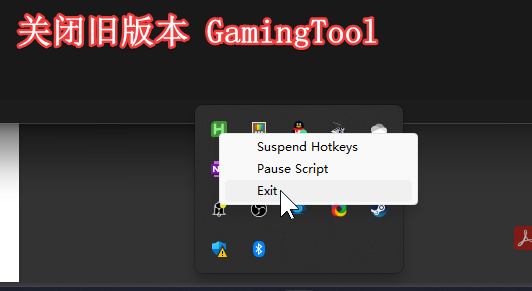
\includegraphics[width=\textwidth]{docs/assets/update/close_gamingtool.png}
%     \caption{关闭 \lstinline{GamingTool}}
% \end{figure}

% 下载新版本压缩包。Windows 会将从网络上下载的文件设置为锁定状态,需要在属性中解除锁定。

% \begin{figure}[H]
%     \Centering
%     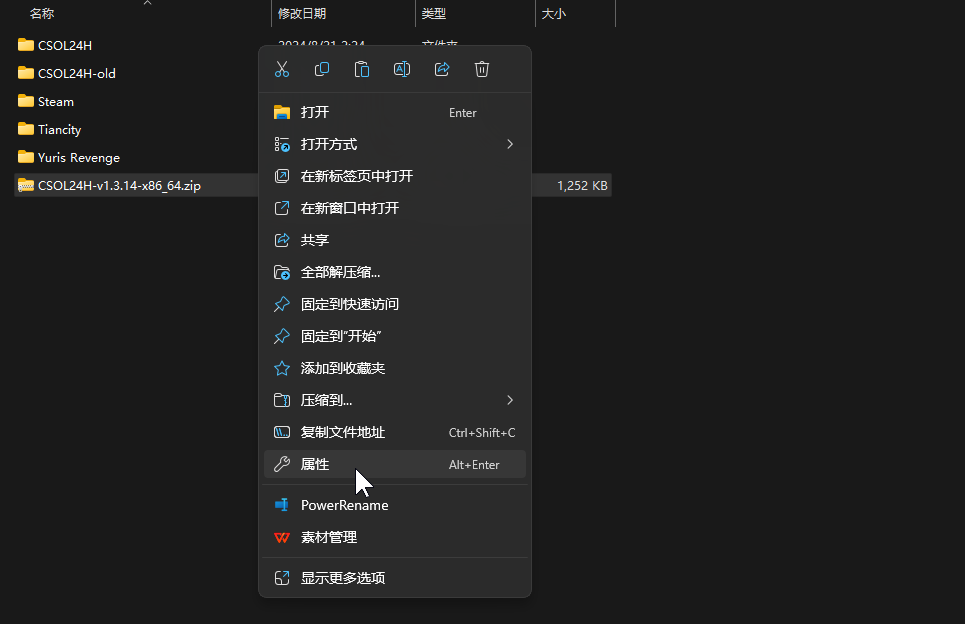
\includegraphics[width=\textwidth]{docs/assets/update/unlock_00.png}
%     \caption{点击“属性”}
% \end{figure}

% \begin{figure}[H]
%     \Centering
%     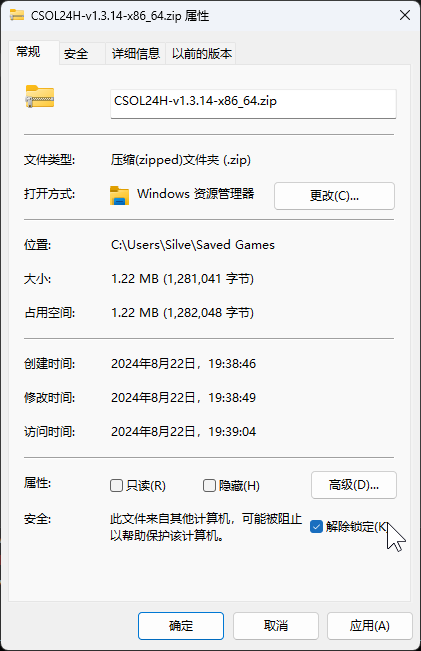
\includegraphics[width=\textwidth]{docs/assets/update/unlock_01.png}
%     \caption{解除锁定}
% \end{figure}

% 解压缩新版集成工具。

% \begin{figure}[H]
%     \Centering
%     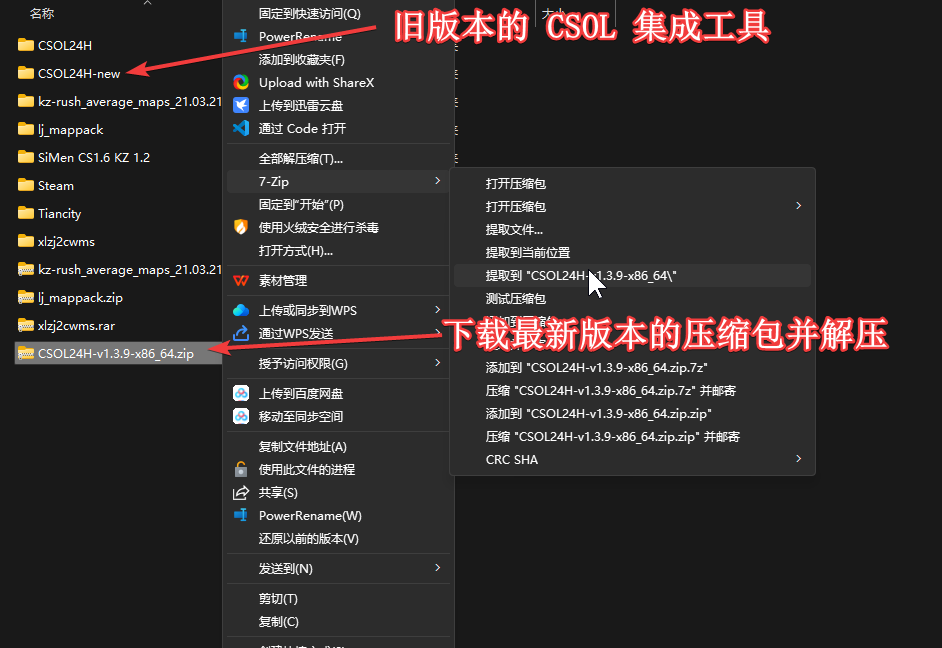
\includegraphics[width=\textwidth]{docs/assets/update/extract_new_version.png}
%     \caption{解压新版本压缩包}
% \end{figure}

% \subsection{从旧版更新到 v1.3.15 及之前版本}

% 本节将以更新旧版本工具到 v1.3.14 版本为例向您说明更新本工具的步骤。

% 打开您原先使用的旧版集成工具目录(图中 \lstinline{CSOL24H-old})和解压后的新版本集成工具目录(图中 \lstinline{CSOL24H-v1.3.14-x86_64})。
% 分别打开它们的 \lstinline{lua} 目录。

% \begin{figure}[H]
%     \Centering
%     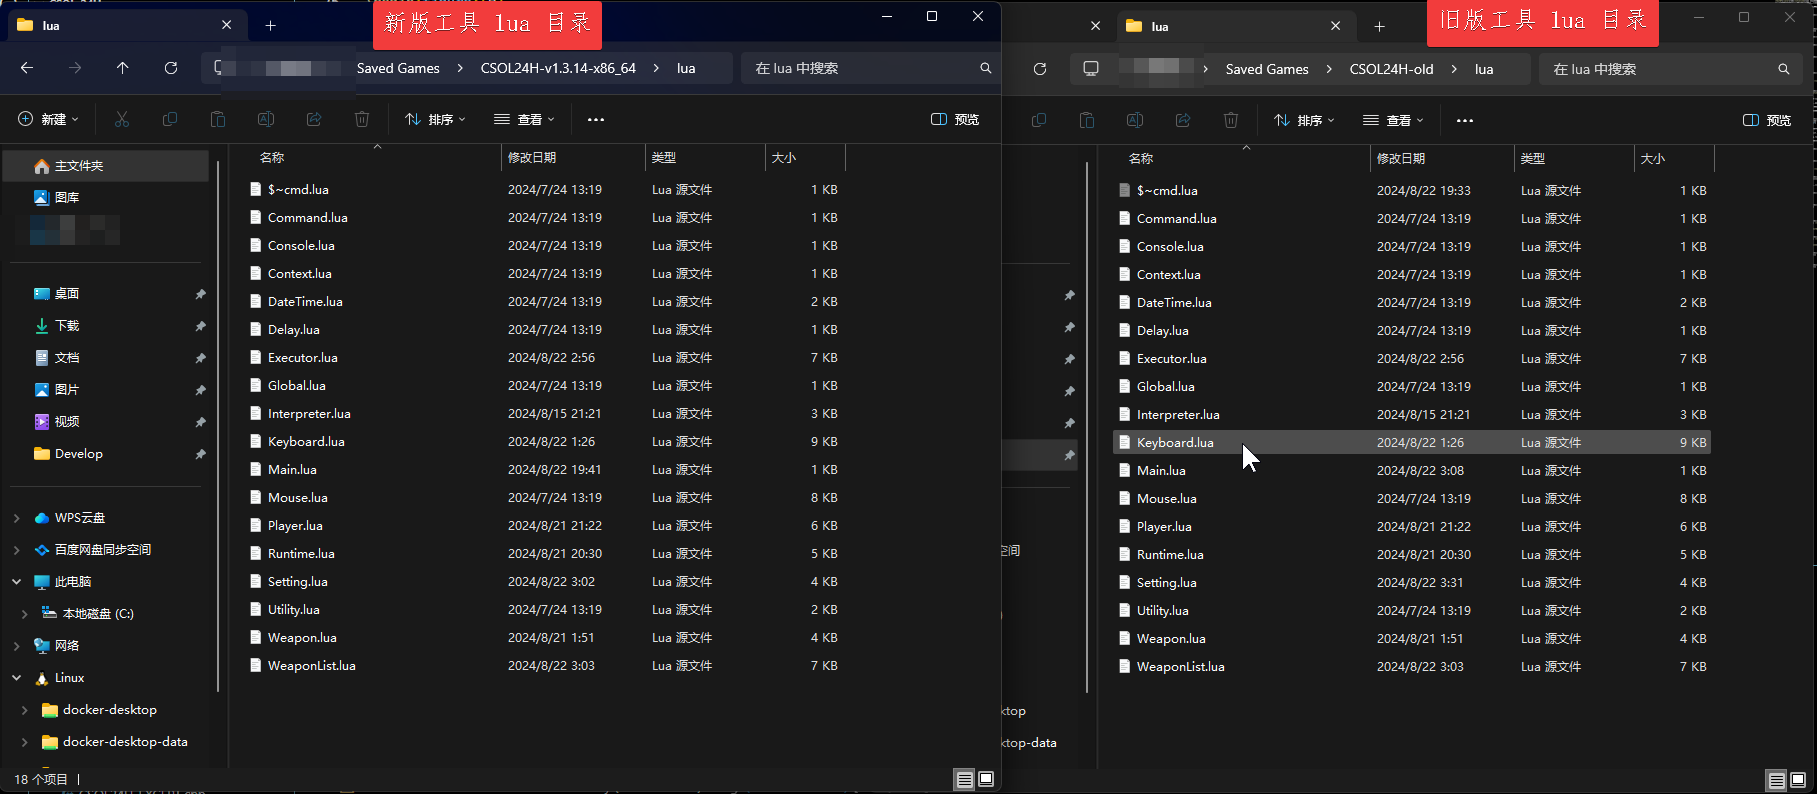
\includegraphics[width=\textwidth]{docs/assets/update/replace_00.png}
%     \caption{进入新旧版本集成工具的 \lstinline{lua} 目录}
% \end{figure}

% 在 Powershell 中运行 \lstinline{CSOL24H-v1.3.14-x86_64} 目录下的 \lstinline{install.ps1} 以配置新版本工具 Lua 模块运行路径。

% \begin{figure}[H]
%     \Centering
%     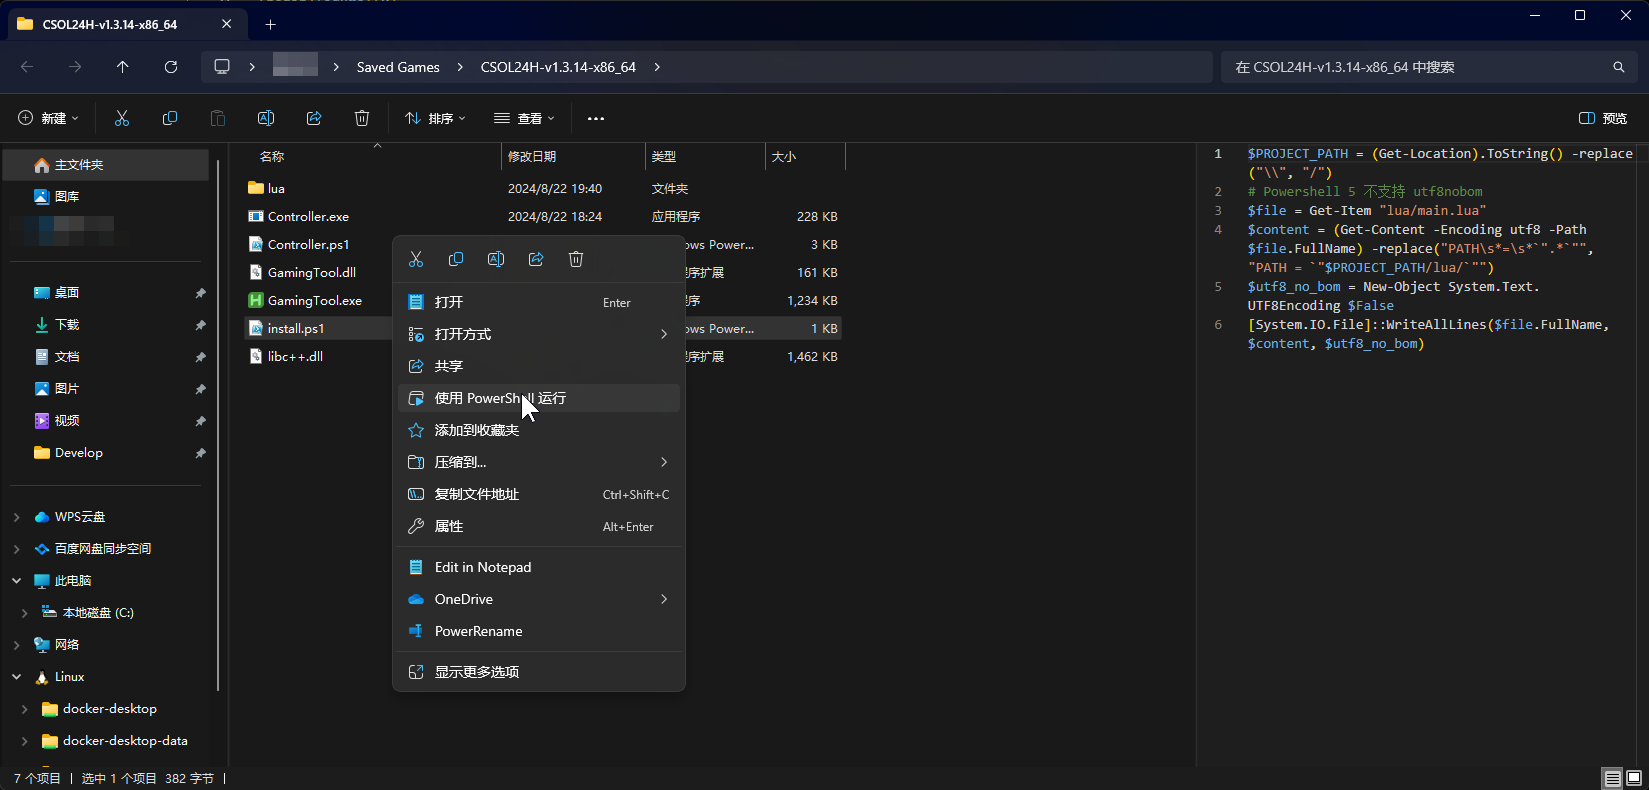
\includegraphics[width=\textwidth]{docs/assets/update/run_install.png}
%     \caption{运行新版本的 \lstinline{install.ps1},配置 Lua 模块运行路径}
% \end{figure}

% \textbf{\color{red} 先对比您的配置文件和新版本压缩包中给出的示例配置文件(\lstinline{Setting.lua} 和 \lstinline{WeaponList.lua}),查看是否有缺漏的配置。
% 若有新增内容(新增内容会予以注明),则将其根据您的实际情况结合文档说明添加到您的原有的配置文件中。}

% 例如,通过对比可以看出 v1.3.14 版本对配置文件 \lstinline{Setting.lua} 作出了更新,按照下图标注的方式,将此更新同步到您的配置文件中(坐标位置需自行调整,详见后文,此时导入是为了正常使用模式 5)。

% \begin{figure}[H]
%     \Centering
%     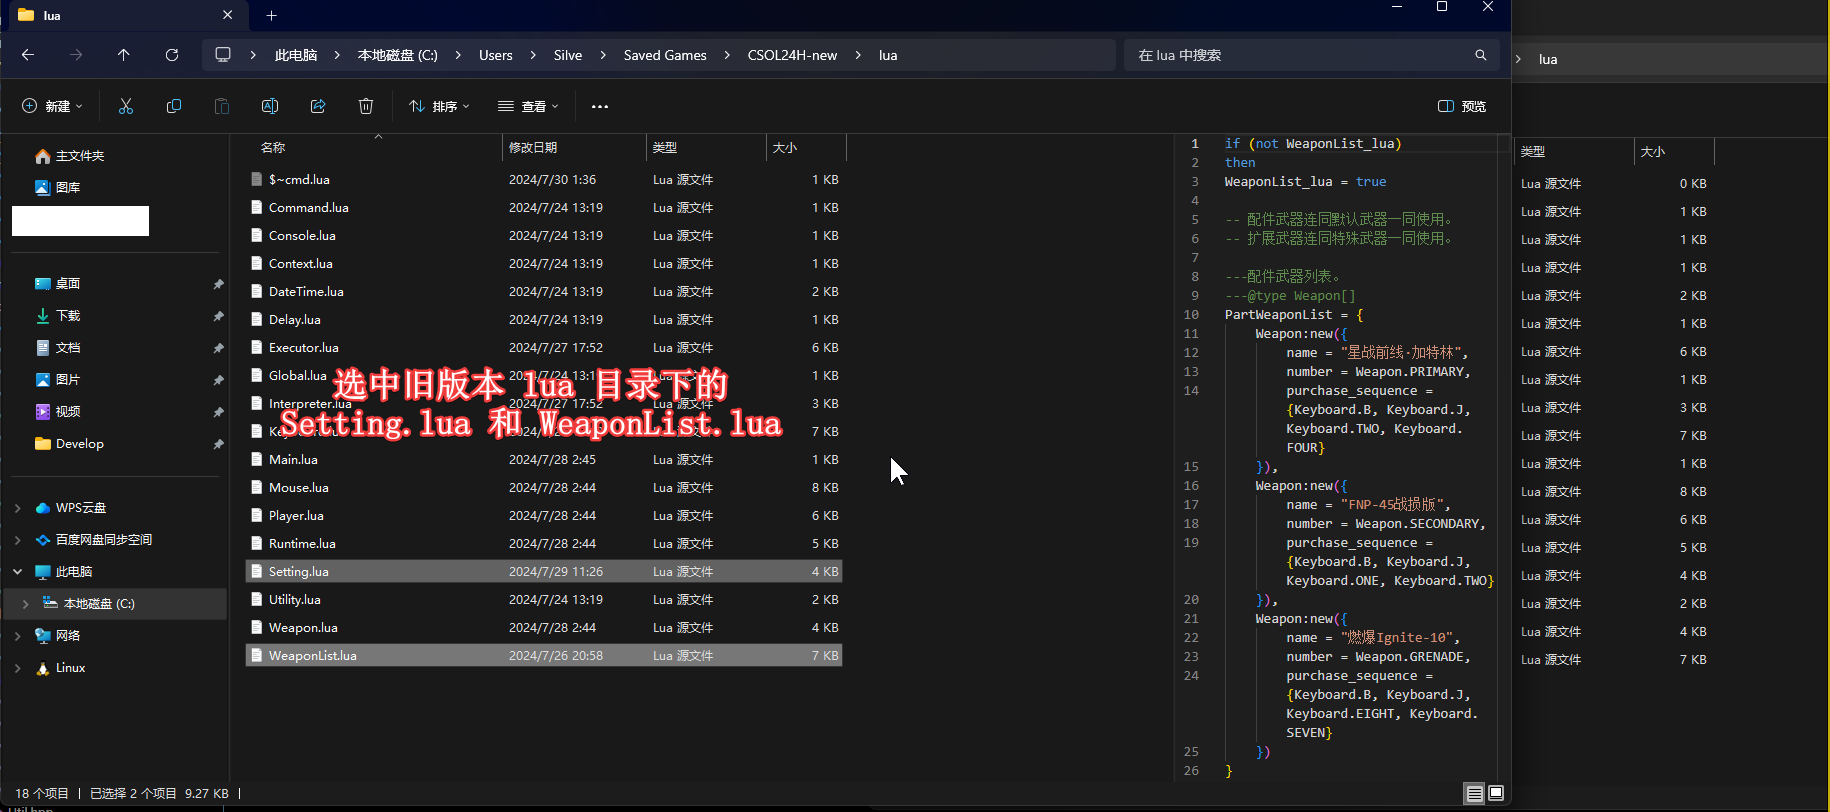
\includegraphics[width=\textwidth]{docs/assets/update/replace_01.png}
%     \caption{对比您的配置文件和新版样例配置文件}
% \end{figure}

% \begin{figure}[H]
%     \Centering
%     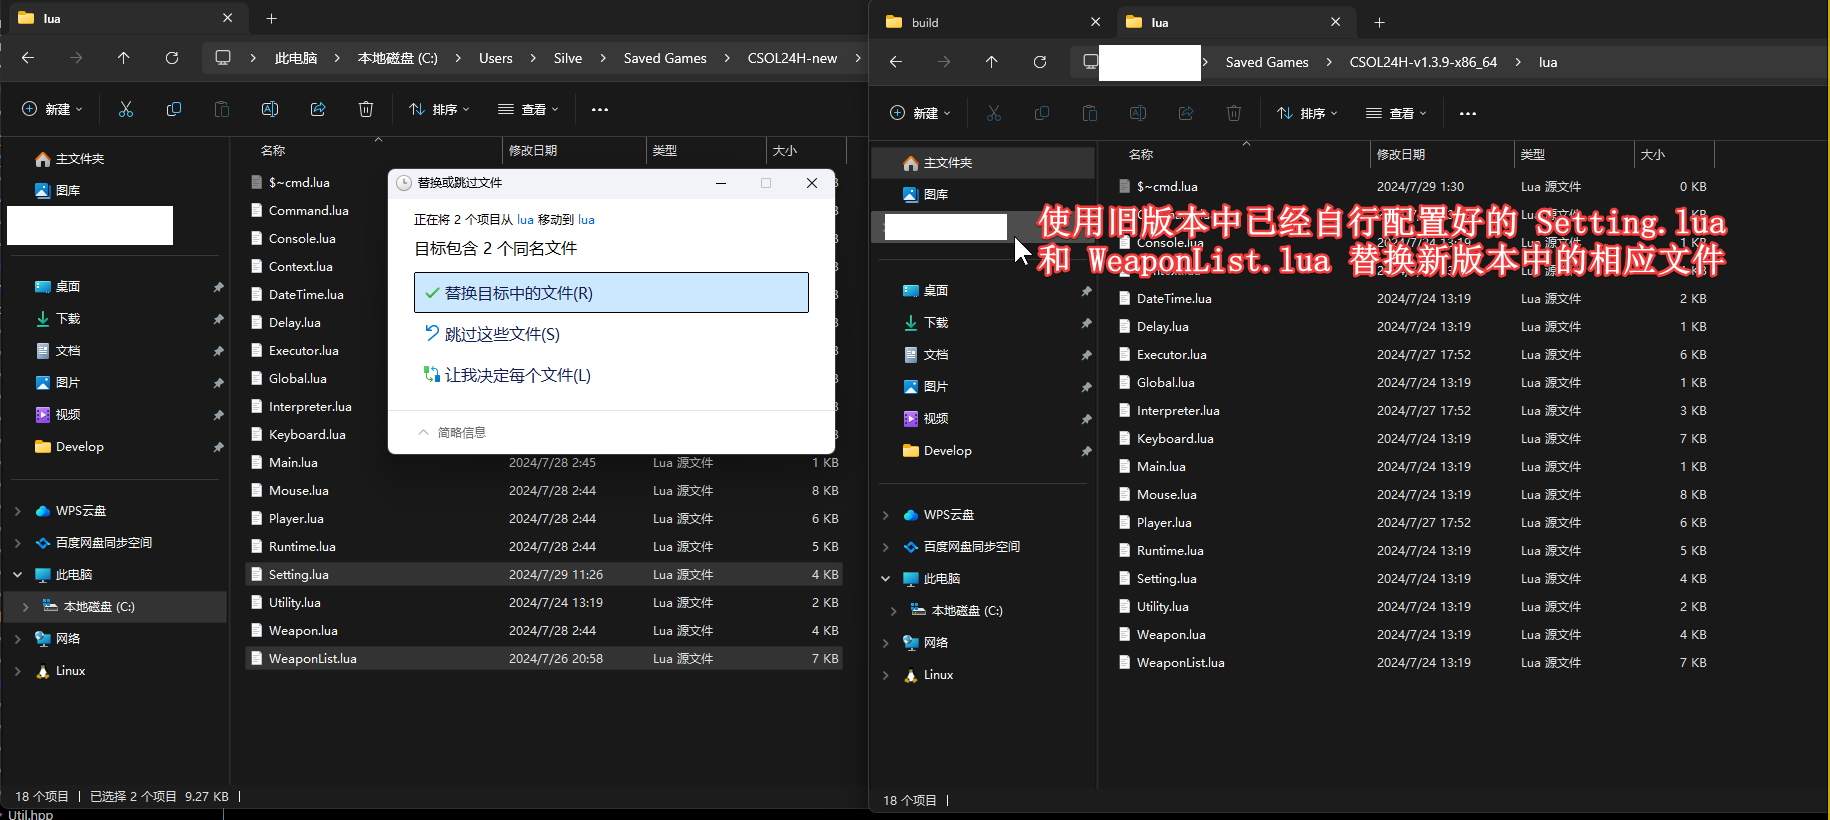
\includegraphics[width=\textwidth]{docs/assets/update/replace_02.png}
%     \caption{将 \lstinline{Setting.lua} 中的更新的部分复制到您自己的配置文件中}
% \end{figure}

% 保存更改后,选中旧版本集成工具使用的 \lstinline{Setting.lua} 和 \lstinline{WeaponList.lua} 两个配置文件,拖拽到新版本集成工具的 \lstinline{lua} 目录中进行替换。

% \begin{figure}[H]
%     \Centering
%     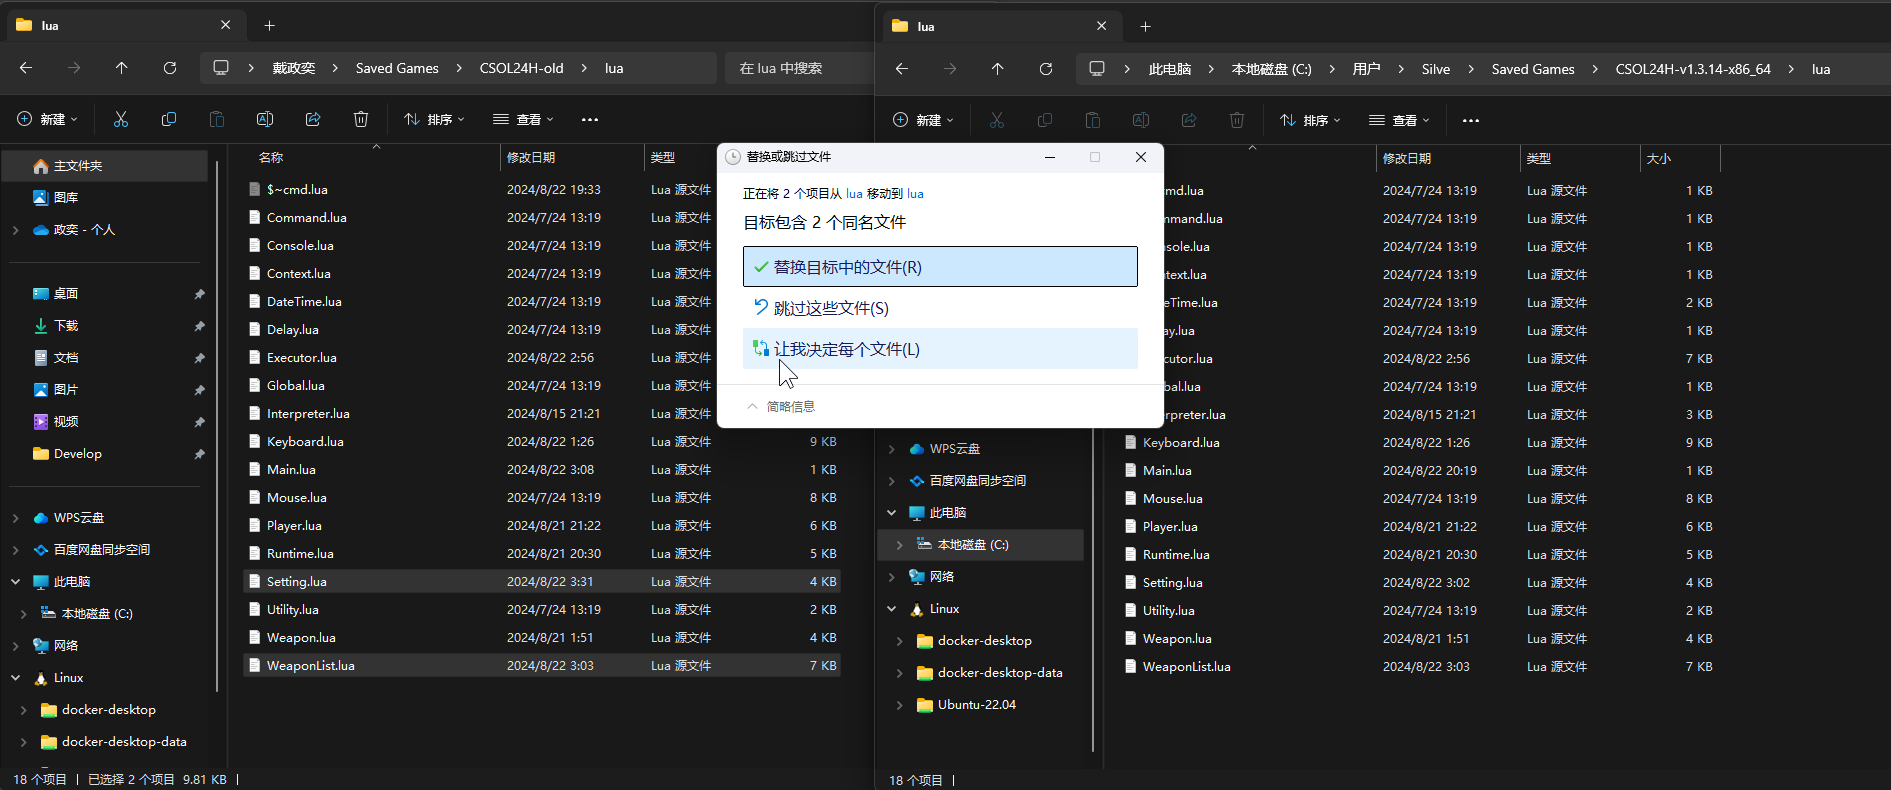
\includegraphics[width=\textwidth]{docs/assets/update/replace_03.png}
%     \caption{替换配置文件}
% \end{figure}

% 替换完成后,打开罗技软件(确保以管理员权限运行),导入新版本集成工具 \lstinline{lua} 目录下的 \lstinline{Main.lua} 文件。

% \begin{figure}[H]
%     \Centering
%     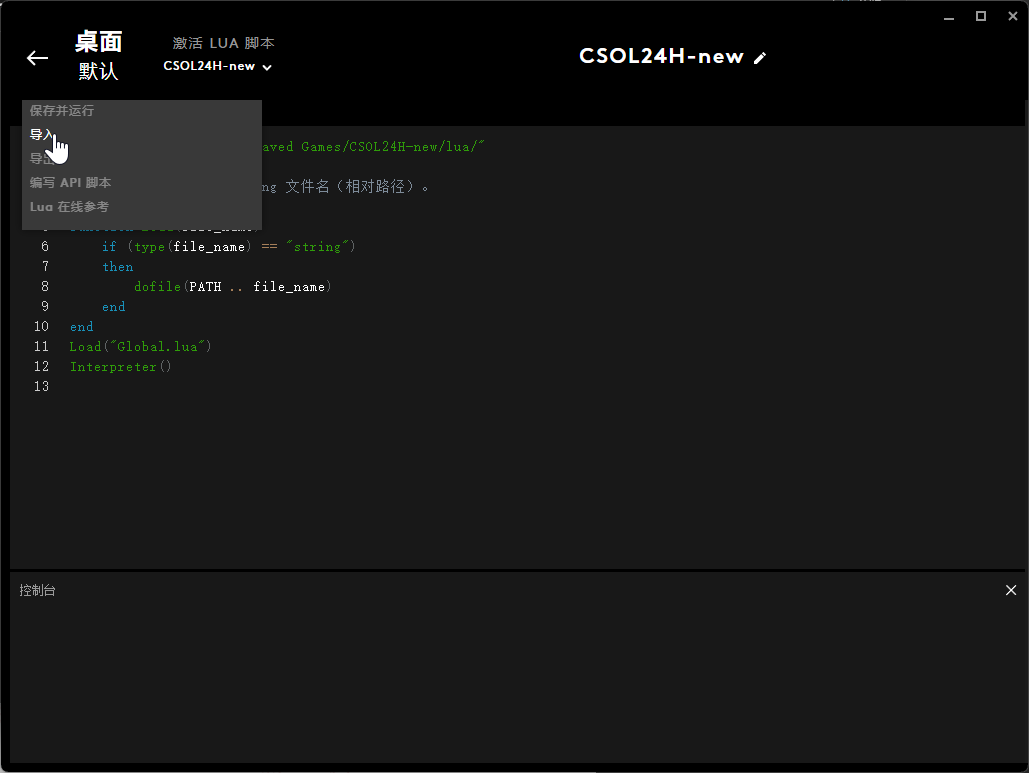
\includegraphics[width=\textwidth]{docs/assets/update/import_main_00.png}
%     \caption{点击“导入”}
% \end{figure}

% \begin{figure}[H]
%     \Centering
%     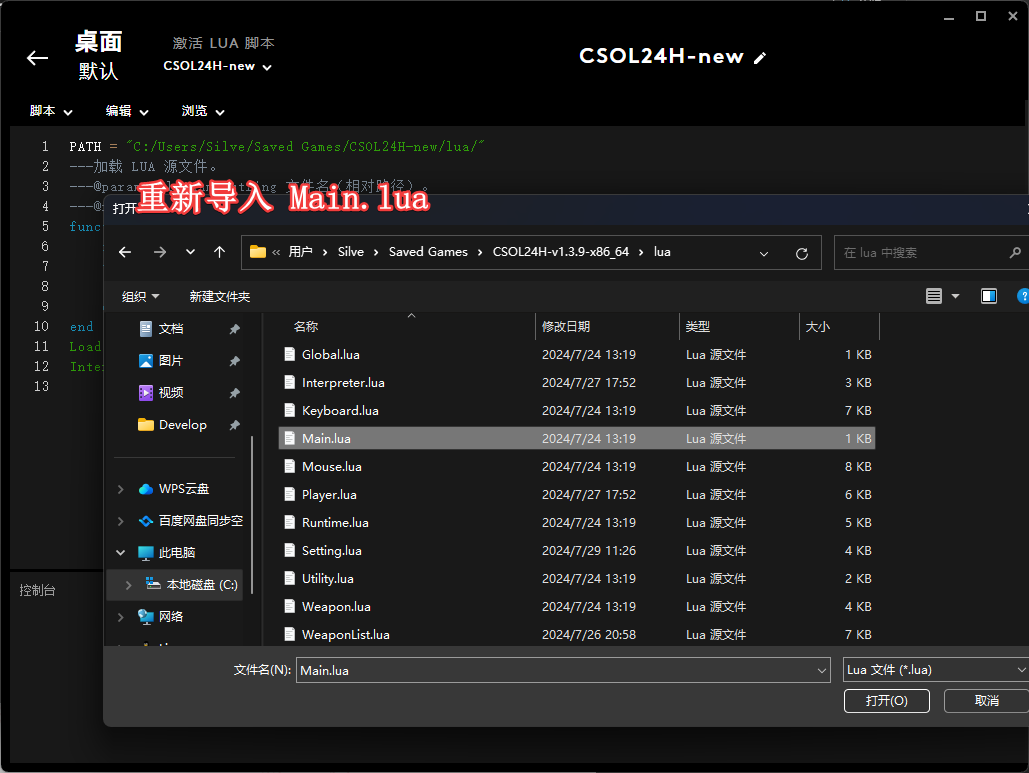
\includegraphics[width=\textwidth]{docs/assets/update/import_main_01.png}
%     \caption{导入 \lstinline{Main.lua}}
% \end{figure}

% 然后,保存并运行导入的 Lua 源文件。

% \begin{figure}[H]
%     \Centering
%     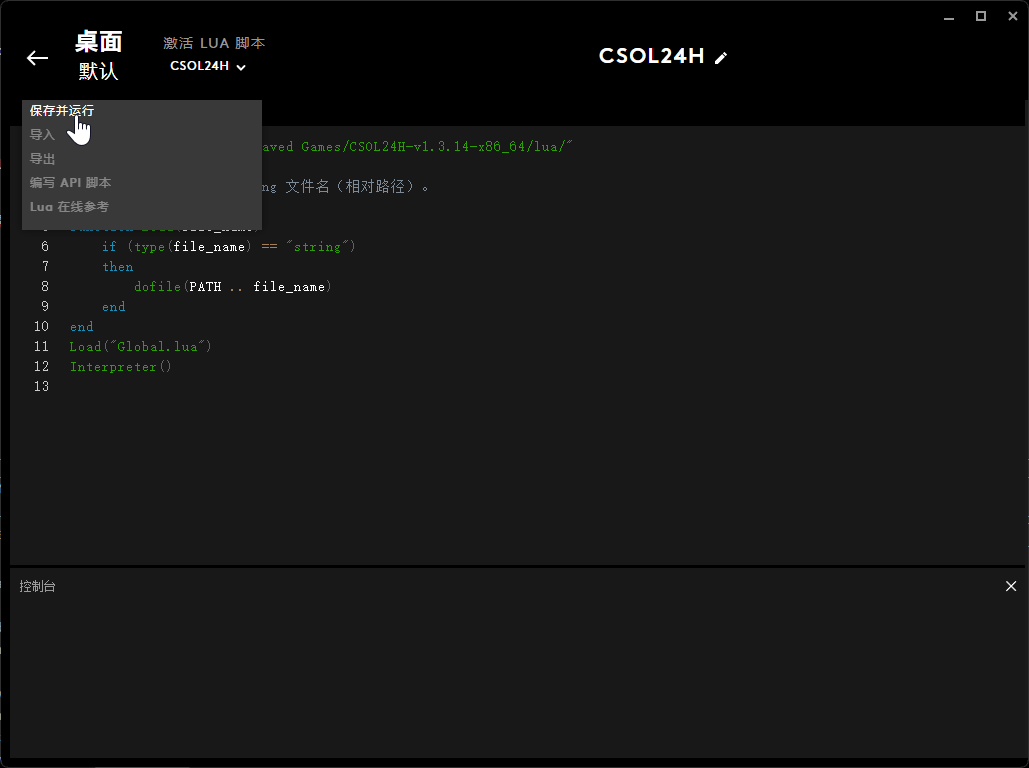
\includegraphics[width=\textwidth]{docs/assets/update/save_and_run_00.png}
%     \caption{点击“保存并运行”(也可以按 \lstinline{Ctrl} \lstinline{S} 保存)}
% \end{figure}

% 看到您的配置文件导入信息即表示成功。

% \begin{figure}[H]
%     \Centering
%     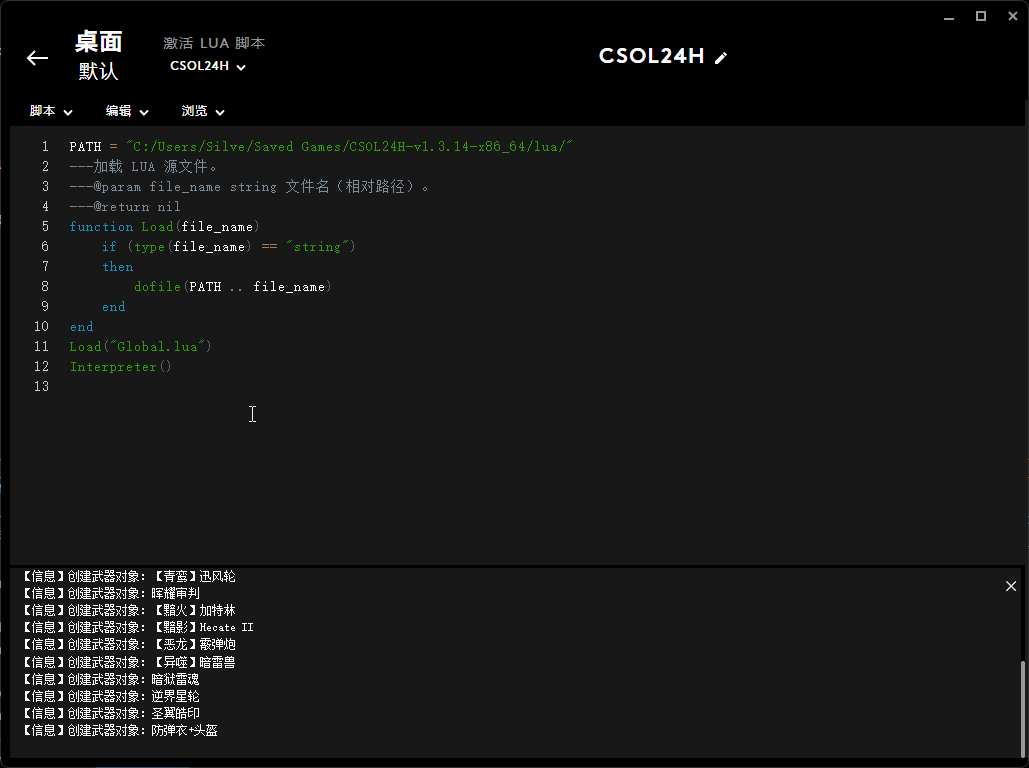
\includegraphics[width=\textwidth]{docs/assets/update/save_and_run_01.png}
%     \caption{点击“保存并运行”(也可以按 \lstinline{Ctrl} \lstinline{S})}
% \end{figure}

% 注意,v1.3.14 及之后的版本提供的配置文件样例中标明了配置时需要参考的手册章节号以便查阅(图 \ref{ch5fig-section-number-in-conf})。

% \begin{figure}[H]
%     \Centering
%     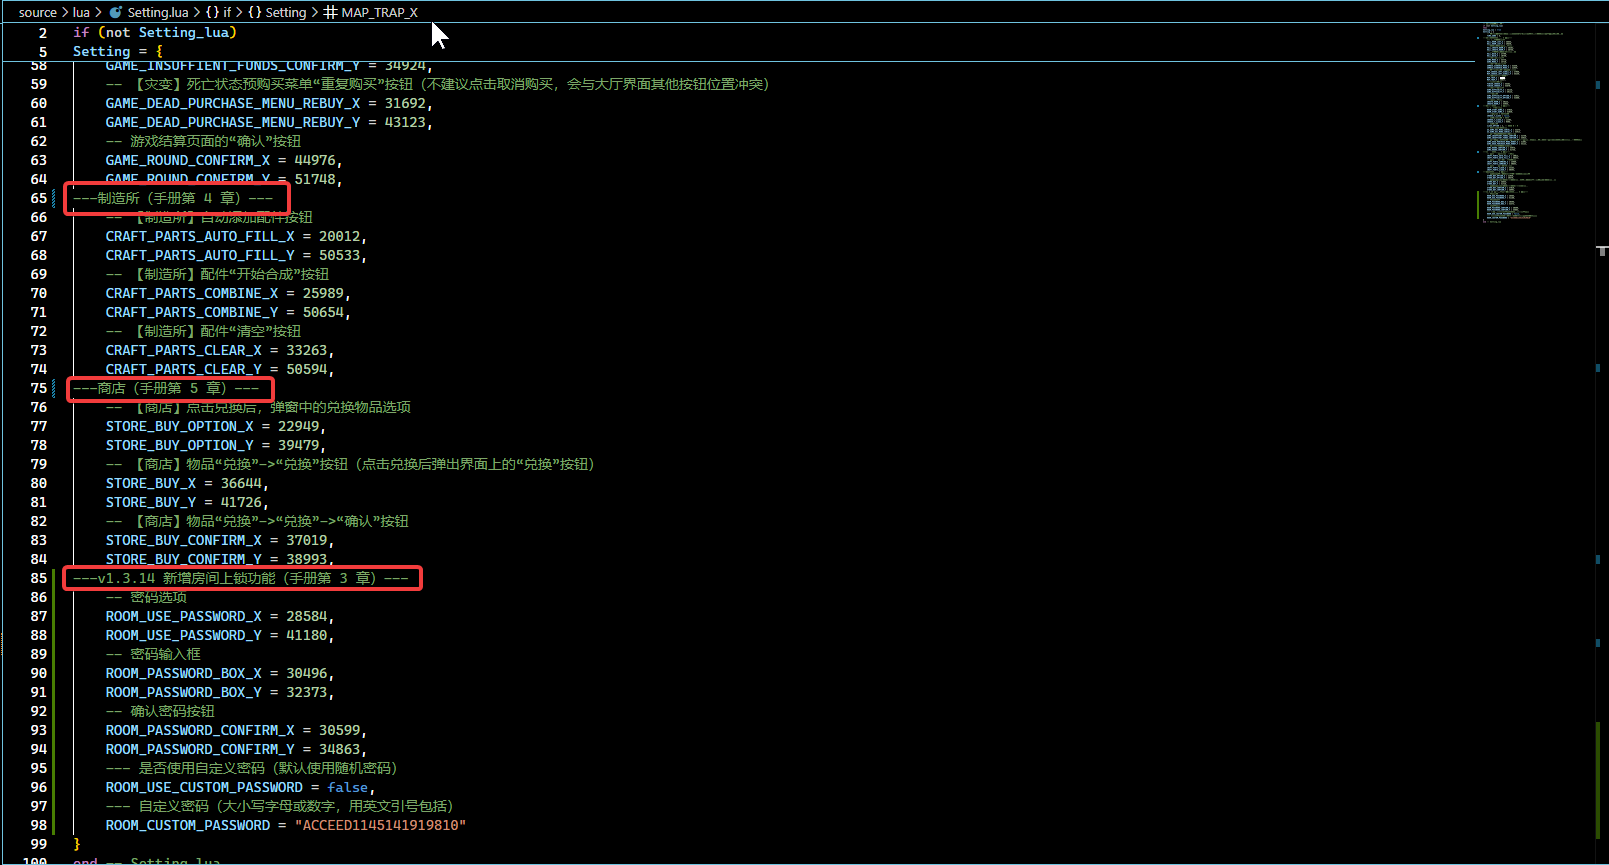
\includegraphics[width=\textwidth]{docs/assets/update/section_number_in_conf.png}
%     \caption{v1.3.14 配置文件样例中标注了配置时需要参考的手册章节号}
%     \label{ch5fig-section-number-in-conf}
% \end{figure}

% 然后,运行 \lstinline{GamingTool} 和 \lstinline{Controller}。

% \begin{figure}[H]
%     \Centering
%     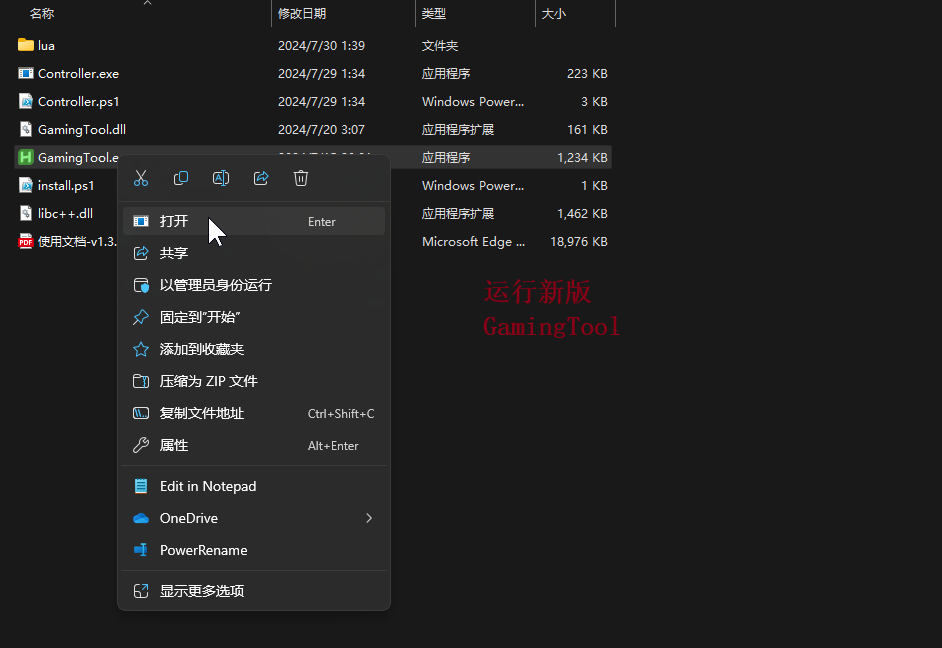
\includegraphics[width=\textwidth]{docs/assets/update/run_new_gamingtool.png}
%     \caption{运行 \lstinline{GamingTool}}
% \end{figure}

% \begin{figure}[H]
%     \Centering
%     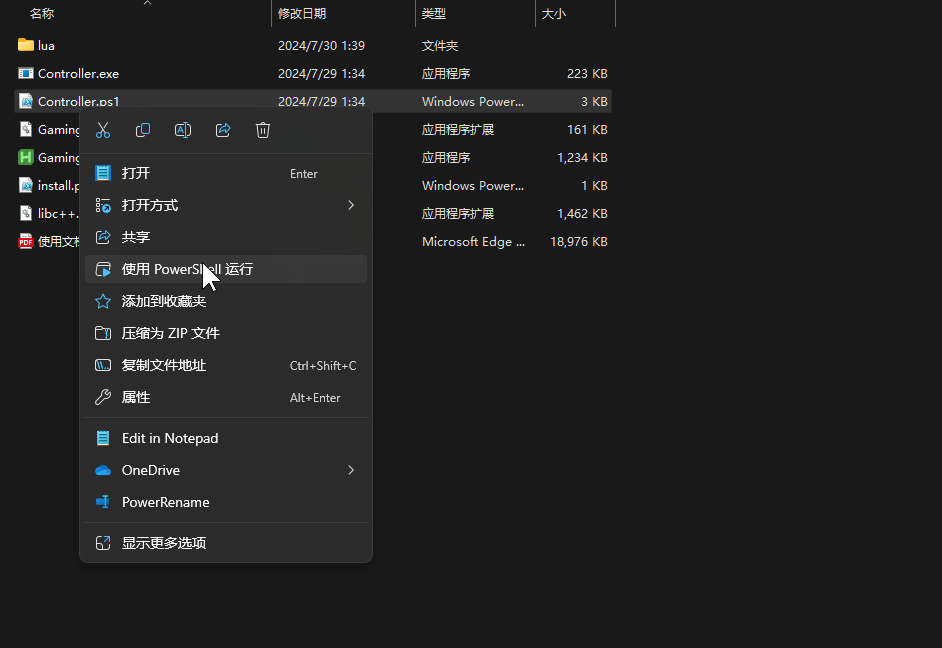
\includegraphics[width=\textwidth]{docs/assets/update/run_new_controller.png}
%     \caption{运行 \lstinline{Controller}}
% \end{figure}

% \textbf{\color{red} 本例中,\lstinline{Setting.lua} 中新增了需要配置的坐标(章节号已经标注)。找到相应的章节,使用模式 5 根据说明配置这些坐标即可。}

% \begin{figure}[H]
%     \Centering
%     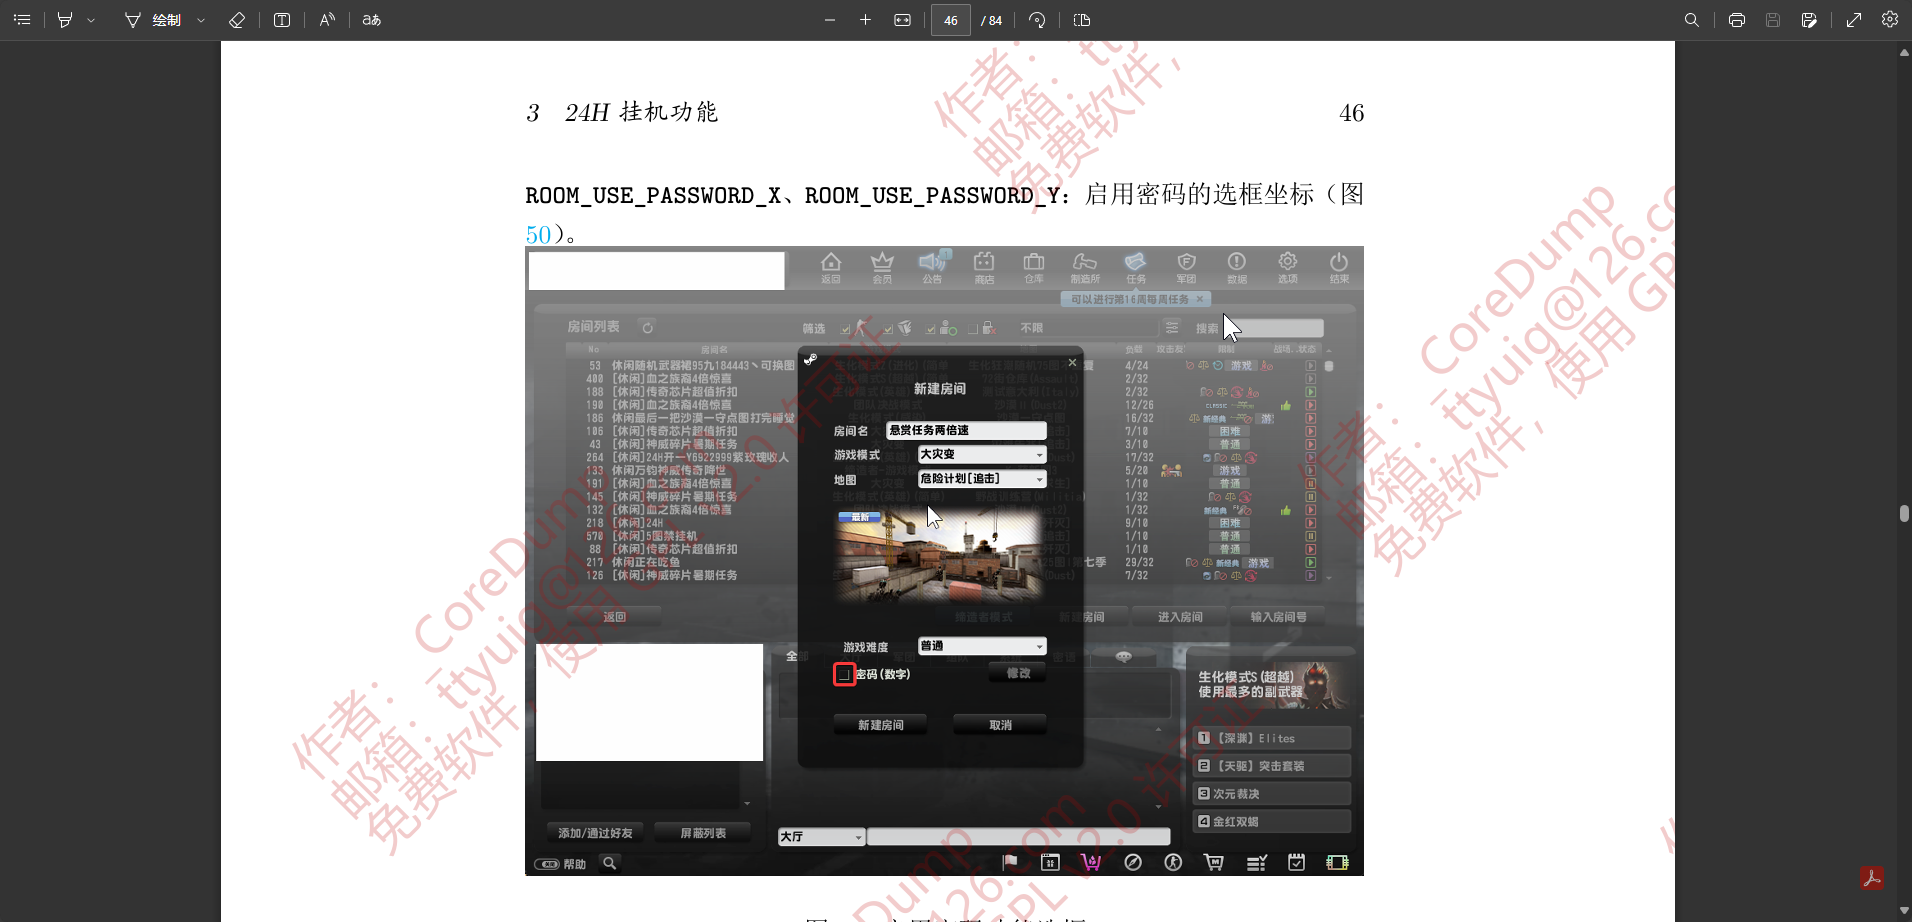
\includegraphics[width=\textwidth]{docs/assets/update/config_new_positions_00.png}
%     \caption{配置新坐标}
% \end{figure}

% \begin{figure}[H]
%     \Centering
%     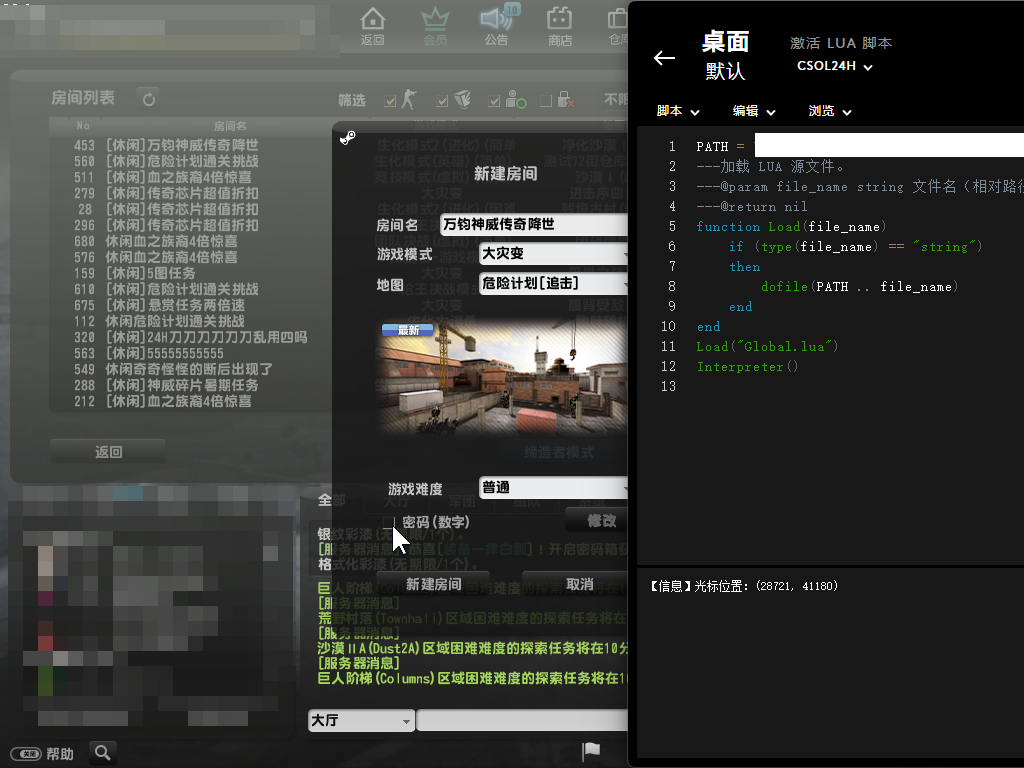
\includegraphics[width=\textwidth]{docs/assets/update/config_new_positions_01.png}
%     \caption{配置新坐标}
% \end{figure}

% \begin{figure}[H]
%     \Centering
%     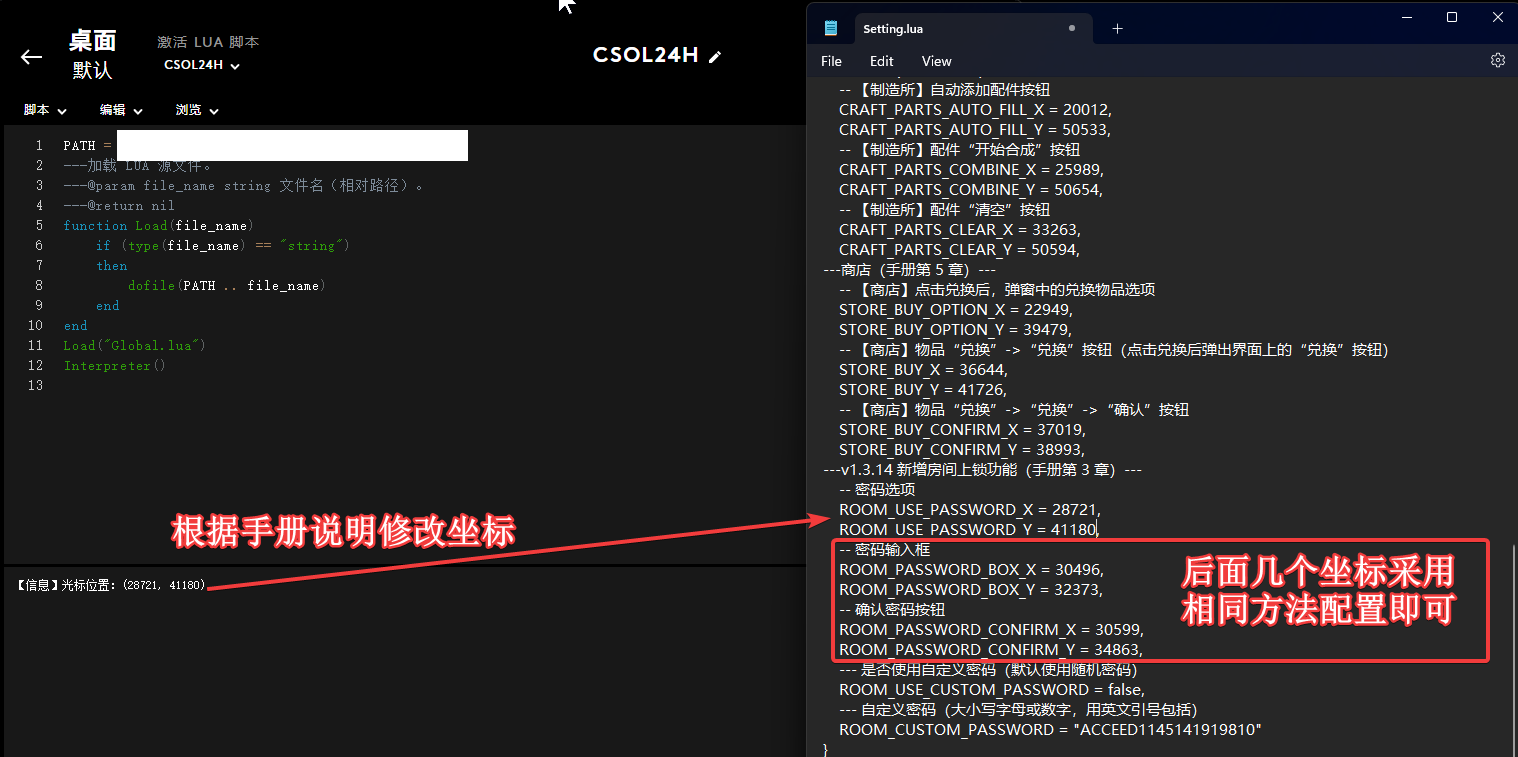
\includegraphics[width=\textwidth]{docs/assets/update/config_new_positions_02.png}
%     \caption{配置新坐标}
% \end{figure}

% 配置完成并保存修改后,勿忘在罗技软件中重新保存使修改后的配置生效(由于 \lstinline{Main.lua} 没有被修改,此时无需重复导入 \lstinline{Main.lua},只需要点击“保存并运行”即可)。

% \subsection{更新到 v1.3.16 及以上版本}

下载新版集成工具压缩包并解压后(注意需解除锁定),在 Powershell 中运行 \lstinline{install.ps1}(运行前需注意是否已经按照第一章所属步骤修改 Powershell 执行策略)。

在罗技软件中导入新版本集成工具中的 \lstinline{Main.lua}。

在浏览器中打开网页 \lstinline{Setting.html}。

在网页最下方点击“导入”,将您的旧版集成工具使用的 \lstinline{Setting.lua} 文件导入。

\begin{figure}[H]
    \Centering
    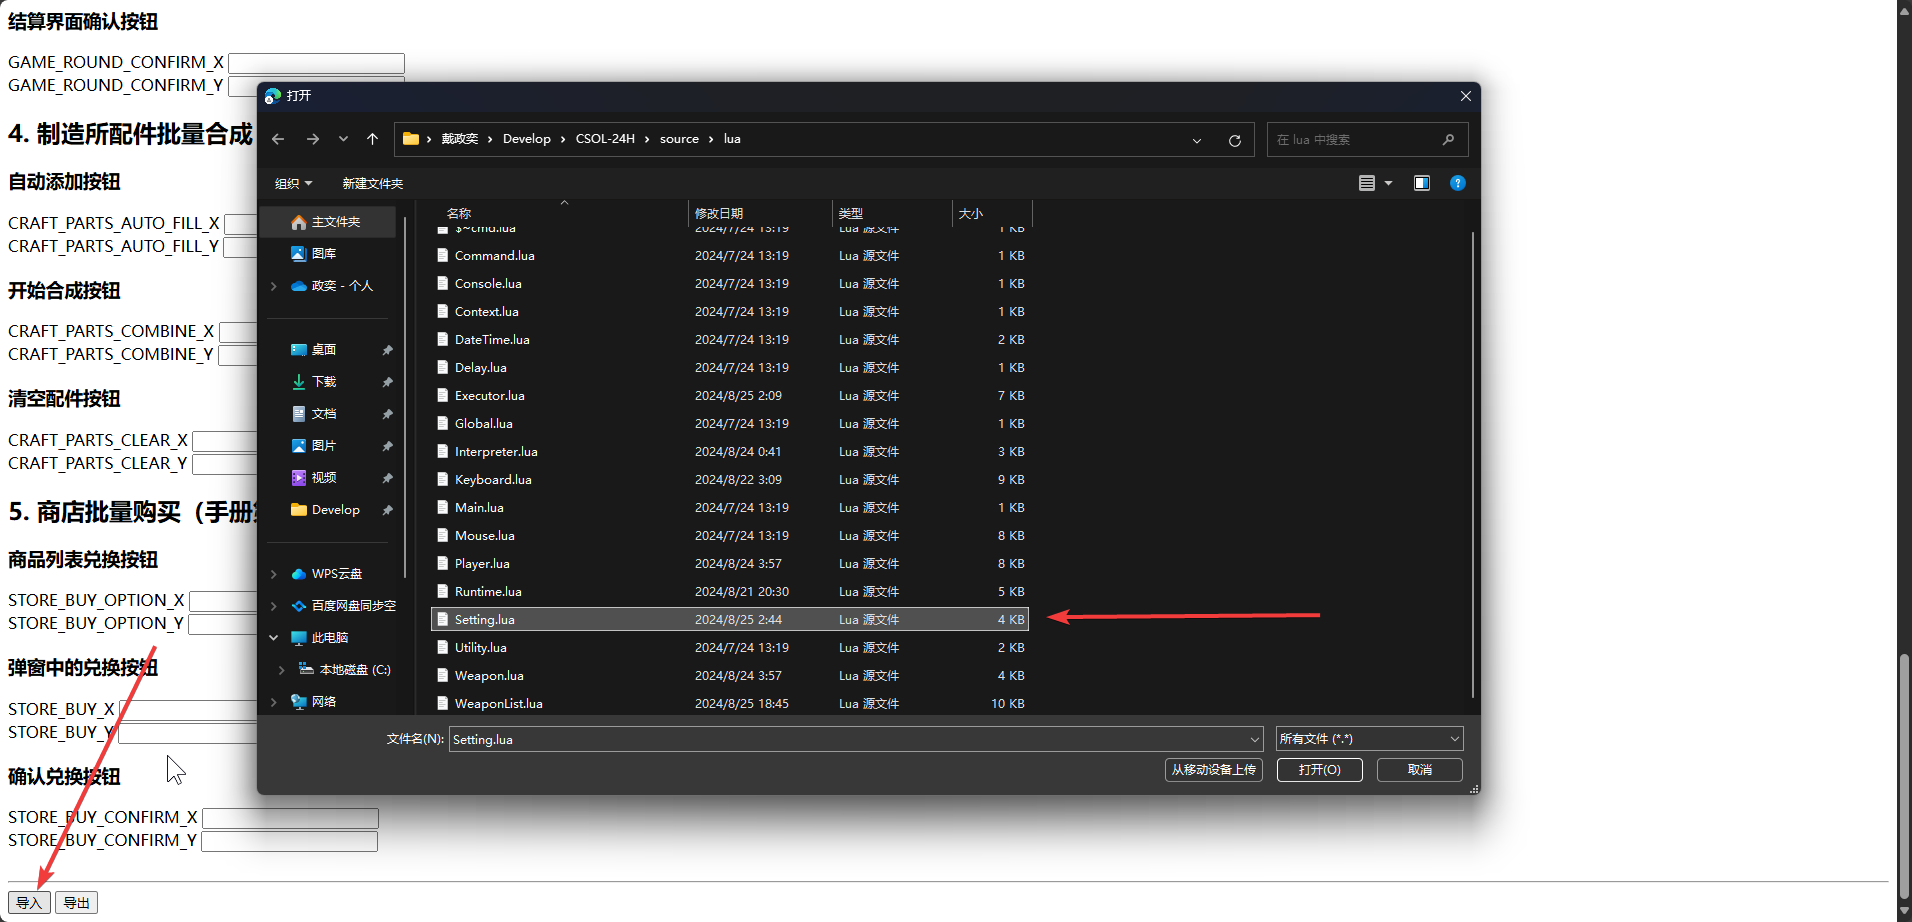
\includegraphics[width=\textwidth]{docs/assets/update/import_setting}
    \caption{导入旧版集成工具使用的 \lstinline{Setting.lua}}
\end{figure}

然后,点击“导出”,若存在尚未配置的字段,则网页会弹出提示,根据提示查阅手册填补缺失的字段即可。

\begin{figure}[H]
    \Centering
    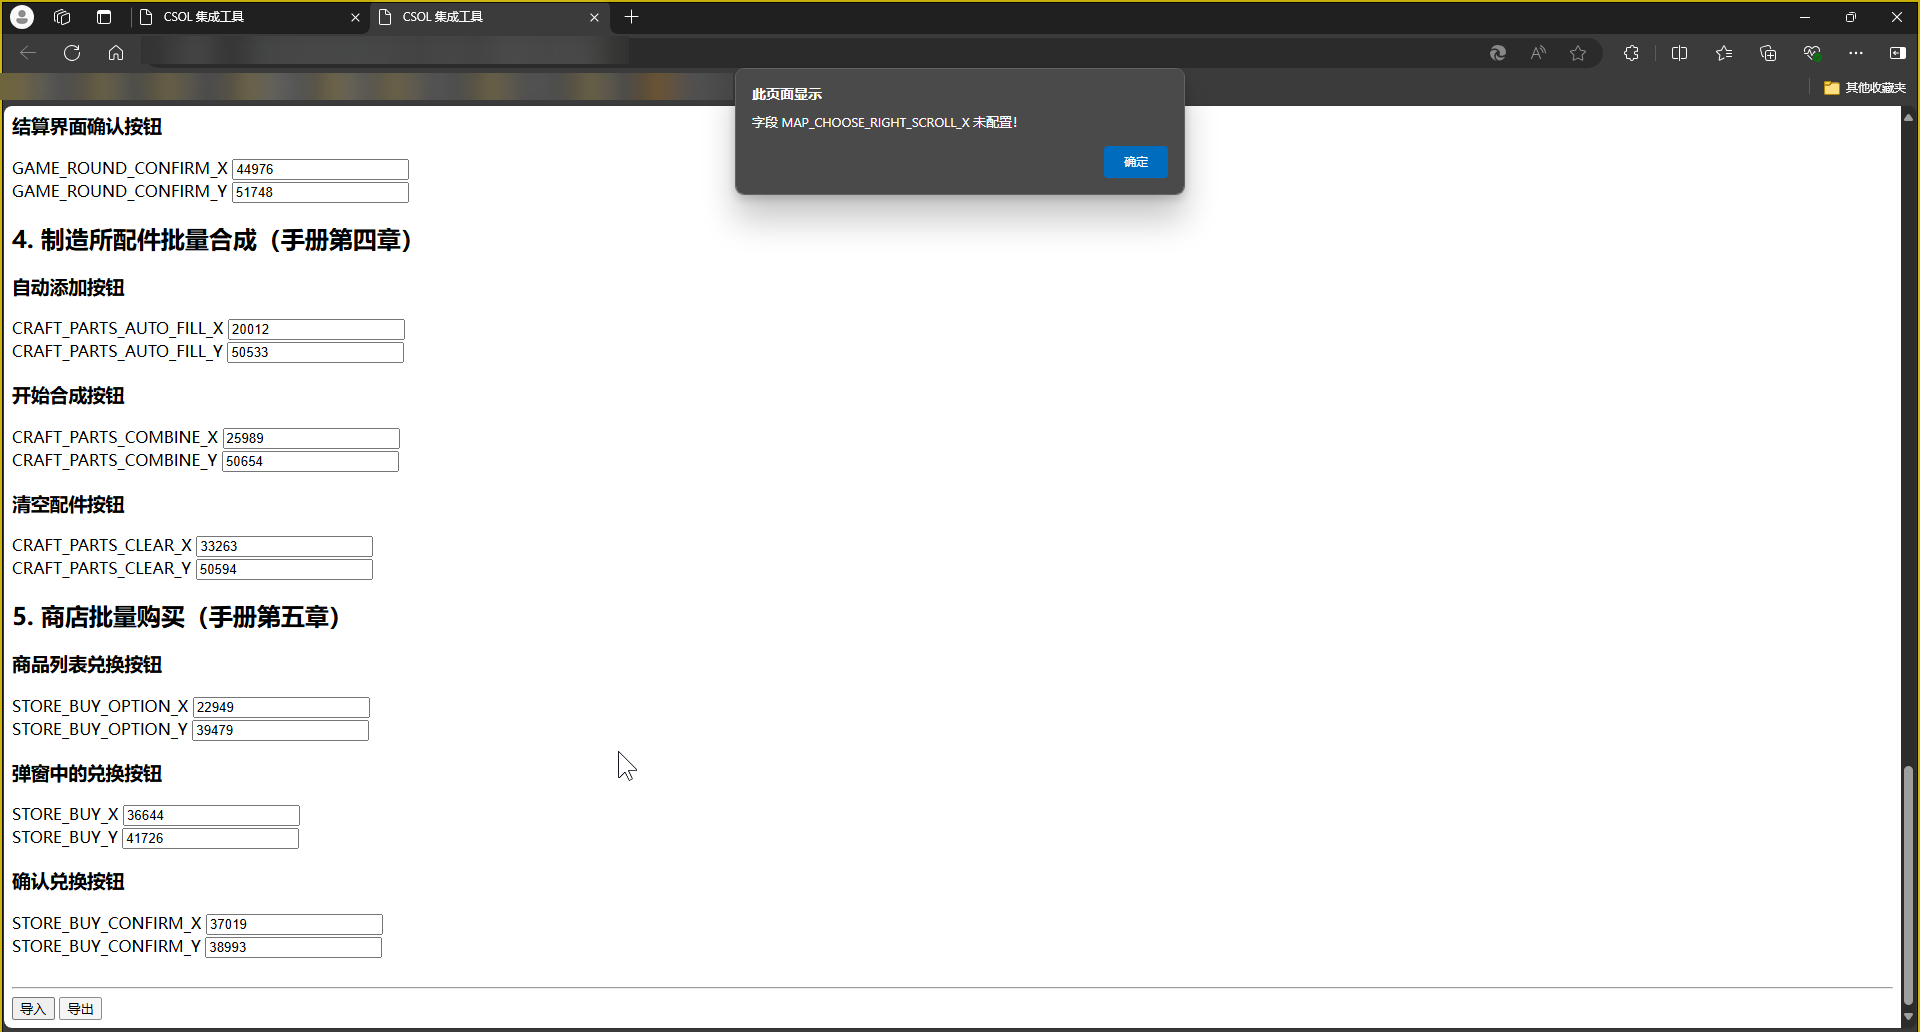
\includegraphics[width=\textwidth]{docs/assets/update/export_error}
    \caption{根据网页提示的信息填补缺失字段}
\end{figure}

填补完成后,导出 \lstinline{Setting.lua} 到新版集成工具的 \lstinline{Executor} 目录下,覆盖原有的 \lstinline{Setting.lua} 文件。

\begin{figure}[H]
    \Centering
    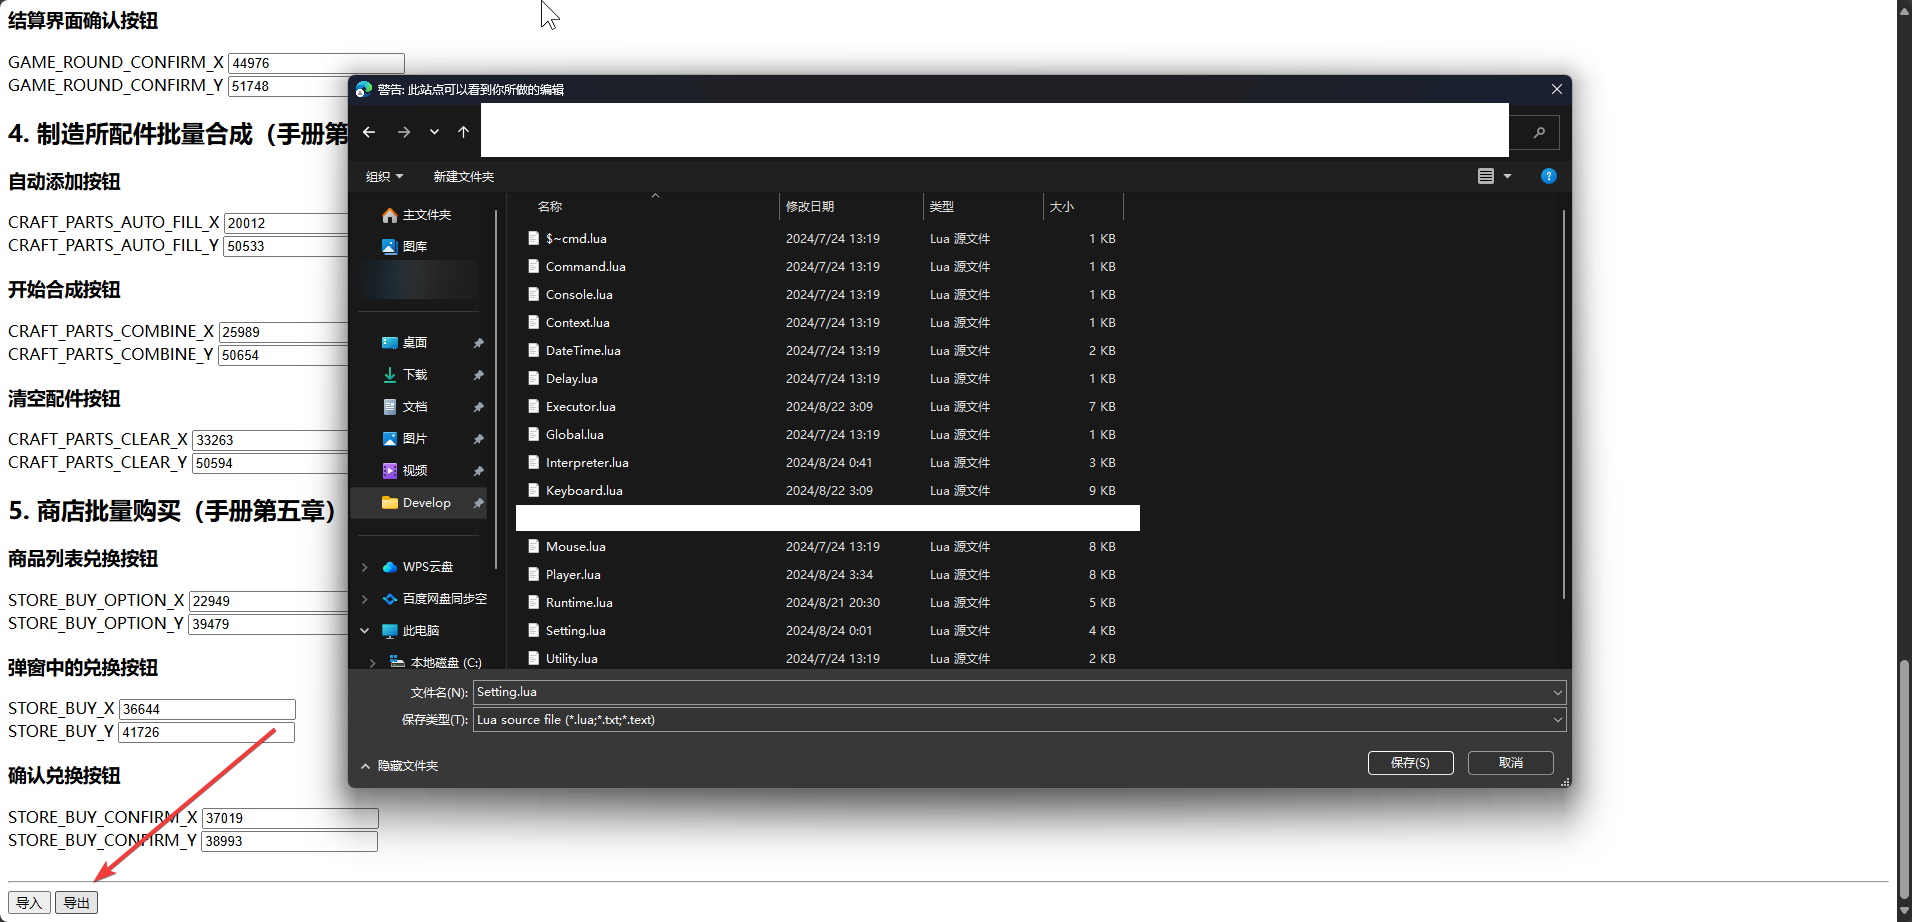
\includegraphics[width=\textwidth]{docs/assets/update/override_setting}
    \caption{导出 \lstinline{Setting.lua}}
\end{figure}

然后,将旧版集成工具使用的 \lstinline{WeaponList.lua} 文件移动到新版集成工具的 \lstinline{Executor} 目录下,
覆盖原有的 \lstinline{WeaponList.lua} 文件(建议先对比一下看新版工具提供的 \lstinline{WeaponList.lua} 模板中是否新增了内容,不过一般不会有)。
如果需要,可以在浏览器中打开 \lstinline{Weapon.html} 进行武器配置。

在罗技软件中重新导入 \lstinline{Main.lua} 使您的配置生效。

最后,运行新版工具的 \lstinline{Controller} 和 \lstinline{GamingTool} 即可正常使用。